\documentclass[journal]{IEEEtran}

%\usepackage[brazil]{babel}
%\usepackage[T1]{fontenc}

\usepackage{theorem}        %%Lo agregue yo <========================================
\usepackage{algorithmic}        %%Lo agregue yo <========================================

\setcounter{secnumdepth}{7}

\newtheorem{theorem}{Theorem}%[section]
%\newtheorem{acknowledgement}[theorem]{Acknowledgement}
%\newtheorem{algorithm}[theorem]{Algorithm}
%\newtheorem{axiom}[theorem]{Axiom}
%\newtheorem{case}[theorem]{Case}
%\newtheorem{claim}[theorem]{Claim}
%\newtheorem{conclusion}[theorem]{Conclusion}
%\newtheorem{condition}[theorem]{Condition}
%\newtheorem{conjecture}[theorem]{Conjecture}
%\newtheorem{criterion}[theorem]{Criterion}
%\newtheorem{exercise}[theorem]{Exercise}
%\newtheorem{notation}[theorem]{Notation}
%\newtheorem{problem}[theorem]{Problem}
%\newtheorem{proposition}[theorem]{Proposition}
%\newtheorem{remark}[theorem]{Remark}
%\newtheorem{solution}[theorem]{Solution}
%\newtheorem{summary}[theorem]{Summary}

\newtheorem{definition}[theorem]{Definition}
\newtheorem{example}[theorem]{Example}
\newtheorem{lemma}[theorem]{Lemma}
\newenvironment{proof}[1][Proof]{\textbf{#1.} }{\ \rule{0.5em}{0.5em}}
\newtheorem{corollary}[theorem]{Corollary}
\newenvironment{algorithm}[1][Algorithm]{\textbf{#1.} }{}

\usepackage{amssymb}
\usepackage{graphicx}
\usepackage{amsmath}
\usepackage{psfrag}

\usepackage{accents}
%\usepackage[none]{hyphenat}

\hyphenation{bet-ween re-pre-sen-ting} %
\sloppy

\begin{document}

\title{Performance Lower Limit  in an Asymmetric Binary CEO Problem}


\author{---------- ---------- ---------- ---------- ---------- %%%%Fernando P. Rivera and Jaime Portugheis
\thanks{Manuscript received XXXX XX, 2014; revised XXXXX XX, 2014.}
\thanks{---------- ---------- ---------- ---------- ---------- ---------- ---------- ---------- ---------- ---------- ---------- }%%%%Fernando P. Rivera is with Department of Communications, State University of Campinas, Campinas, SP, Brazil. Email:fpujaico@decom.fee.unicamp.br. }
\thanks{---------- ---------- ---------- ---------- ---------- ---------- ---------- ---------- ---------- ---------- ---------- }}%%%%Jaime Portugheis   is with Faculty of Technology       , State University of Campinas, Limeira , SP, Brazil. Email:jaime@ft.unicamp.br  .}}

\markboth{IEEE Communications Letters,~Vol.~X,
No.~XX,~XXXXX~XXX}{Shell \MakeLowercase{\textit{et al.}}: Bare
Demo of IEEEtran.cls for Journals}

% make the title area
\maketitle
%%%%%%%\IEEEpeerreviewmaketitle


\begin{abstract}
This paper proposes a method for the calculus of performance lower limit in 
decoding of binary CEO problem. 
Here is analyzed the case when,  over a set of M correlated observed sources, the 
probabilities between these and the unknown source are different.

\end{abstract}


\IEEEpeerreviewmaketitle
%%%%%%%%%%%%%%%%%%%%%%%%%%%%%%%%%%%%%%%%%%%%%%%%%%%%%%%%%%%%%%%%%%%%%%%%%%%%%%%%%%%%%%%
%%%%%%%%%%%%%%%%%%%%%%%%%%%%%%%%%%%%%%%%%%%%%%%%%%%%%%%%%%%%%%%%%%%%%%%%%%%%%%%%%%%%%%%
%%%%%%%%%%%%%%%%%%%%%%%%%%%%%%%%%%%%%%%%%%%%%%%%%%%%%%%%%%%%%%%%%%%%%%%%%%%%%%%%%%%%%%%
\section{Introduction}
\label{sec:Intro}

\begin{itemize}
 \item the Chief Executive Officer(CEO) problem is defined in \cite{ceooriginal}.
 \item An optimal, maximum a posteriori (MAP), algorithm is defined in \cite{optimal} for a 
binary CEO  problem. Data fusion algorithm.
 \item In \cite{ceobinary1,ceobinary2} one theoretical limit is presented for
the case of symmetric binary CEO problem
\end{itemize}

 
%%%%%%%%%%%%%%%%%%%%%%%%%%%%%%%%%%%%%%%%%%%%%%%%%%%%%%%%%%%%%%%%%%%%%%%%%%%%%%
%%%%%%%%%%%%%%%%%%%%%%%%%%%%%%%%%%%%%%%%%%%%%%%%%%%%%%%%%%%%%%%%%%%%%%%%%%%%%%
%%%%%%%%%%%%%%%%%%%%%%%%%%%%%%%%%%%%%%%%%%%%%%%%%%%%%%%%%%%%%%%%%%%%%%%%%%%%%%
\section{System Model and Definitions} 
\label{sec:SystemModel}



The Fig. \ref{fig:modelo} show the diagram of transmission model used in this 
article. In the figure can be seen a binary source $U_0$, $Pr(U_0=1)=0.5$, that
transmit your information across BSC channels, with error probability 
$Pr(U_m \ne U_0 | U_0)=p_m$, $\forall m \in$ $\{1,$ $2,$ $...,$ $M\}$. In the 
out of these channels we obtain $M$ correlated binary sources $U_m$. Each 
source $U_m$, is a noise version of $U_0$. Thus, is possible to get an approximate
version of $U_0$, called $\hat{U}_0$, using the data of $U_m$. This procedure
is called data fusion.
\begin{figure}[h!bt]
\centering
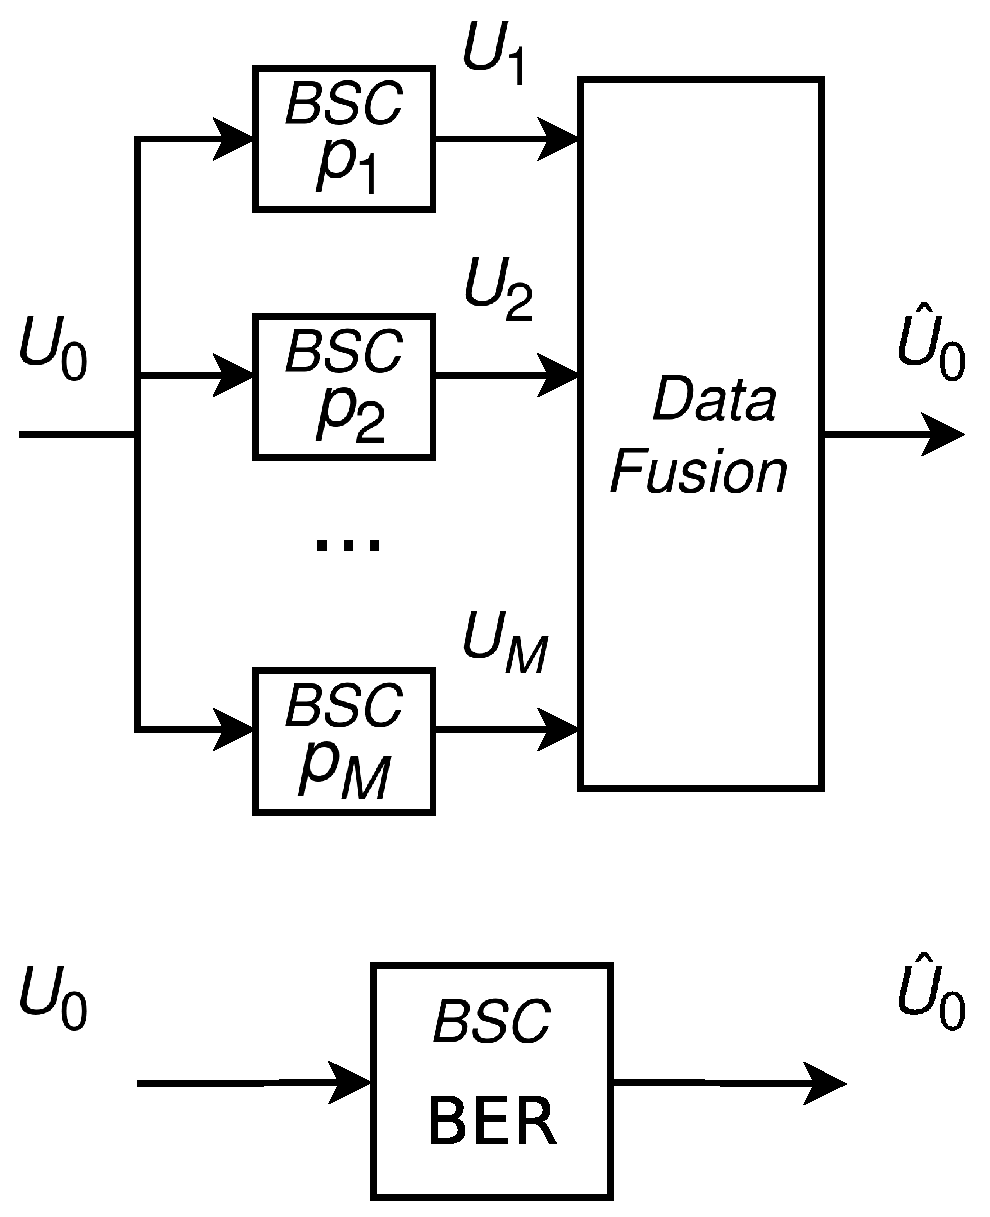
\includegraphics[width=5.0cm]{pujaico1.eps}
\caption{System Model.} \label{fig:modelo}
\end{figure}

%%%%%%%%%%%%%%%%%%%%%%%%%%%%%%%%%%%%%%%%%%%%%%%%%%%%%%%%%%%%%%%%%%%%%%%%%%%%%%
\begin{definition}
 \label{def:omega}
Let $\Omega_m$, $\forall m \in \{1,$ $2,$ $...,$ $M\}$, be a set of correlated 
sources as
\begin{equation}
\label{eq:omega}
 \Omega_m \equiv \{U_i: i \in \mathbf{Z^+}, 1 \leq i \leq m\},
\end{equation}
%with the especial case with $\Omega_0$ equal to null, so that $H(\Omega_0)=0$.

\end{definition}

%%%%%%%%%%%%%%%%%%%%%%%%%%%%%%%%%%%%%%%%%%%%%%%%%%%%%%%%%%%%%%%%%%%%%%%%%%%%%%
\begin{definition}
 \label{def:hb}
The binary entropy is defined as $h_b(\rho)$, so that
\begin{equation}
\label{eq:hb1}
h_b(\rho)=- \rho ~ log_2(\rho) - (1-\rho) ~ log_2(1-\rho).
\end{equation}
If the probability $p_m$ is used, then is defined
\begin{equation}
\label{eq:hi}
h_m \equiv h_b(p_m).
\end{equation}
\end{definition}

 
%%%%%%%%%%%%%%%%%%%%%%%%%%%%%%%%%%%%%%%%%%%%%%%%%%%%%%%%%%%%%%%%%%%%%%%%%%%%%%
%%%%%%%%%%%%%%%%%%%%%%%%%%%%%%%%%%%%%%%%%%%%%%%%%%%%%%%%%%%%%%%%%%%%%%%%%%%%%%
%%%%%%%%%%%%%%%%%%%%%%%%%%%%%%%%%%%%%%%%%%%%%%%%%%%%%%%%%%%%%%%%%%%%%%%%%%%%%%
\section{Optimal Data fusion} 
\label{sec:Optimal}
As is seen in \cite{optimal}, an optimal decision for to get an estimation $\hat{U}^0$ 
in the model of the Fig. \ref{fig:modelo}, is to use a criterion MAP, making 
the quotient
\begin{equation}\label{eq:ceo_0}
L(\mathbf{a})=\frac{P(U^0=1|\Omega^{M}=\mathbf{a})}{P(U^0=0|\Omega^{M}=\mathbf{a})} ,
\end{equation}
where $\mathbf{a}=\{a_1, a_2, ..., a_M\}$ is a m-dimensional binary vector, that 
represent a set of observed values of $U_m$, $\forall m \in$ $\{1,$ $2,$ $...,$ $M\}$.
The  approximation $\hat{U}^0$ of $U^0$, is obtained with
\begin{equation}\label{eq:ceo_1}
\hat{U}^0=
\begin{cases}
1 & \text{ if } L(\mathbf{a}) > 1 \\ 
0 & \text{ if } L(\mathbf{a}) \leq 1
\end{cases}.
\end{equation}
Applying logarithm in equations (\ref{eq:ceo_0}) and (\ref{eq:ceo_1}), these
can be replaced for
\begin{equation}\label{eq:ceo_2}
\phi(\mathbf{a})=\sum_{m=1}^{M}  B_m,
\end{equation}
with $B_m=(2 a_m-1) log({1-p_m}/{p_m})$. $\hat{U}^0$ is obtained with
\begin{equation}\label{eq:ceo_3}
\hat{U}^0=
\begin{cases}
1 & \text{ if } \phi(\mathbf{a}) > 0 \\ 
0 & \text{ if } \phi(\mathbf{a}) \leq 0
\end{cases}.
\end{equation}

\subsection{Performance Lower Limit in Optimal Asymmetric Data Fusion}
How can be seen in \cite{ceobinary1,ceobinary2} a theoretical performance lower 
limit for the case of symmetric binary CEO problem is presented, where 
$Pr(U_m \neq U_0 | U_0)=\rho$, obtaining 
\small
\begin{equation}\label{eq:symlimit}
\begin{matrix}
 Pr(\hat{U}_0 \neq U_0)=\\
\begin{cases}
\frac{1}{2} \binom{M}{\frac{M}{2}}{\rho}^{\frac{M}{2}}{(1-\rho)}^{\frac{M}{2}}+\sum \limits_{k=\frac{M}{2}+1}^{M} \binom{M}{k}{\rho}^{k}{(1-\rho)}^{M-k} & \text{ if } M~even \\ 
\sum \limits_{k=\frac{M+1}{2}}^{M} \binom{M}{k}{\rho}^{k}{(1-\rho)}^{M-k} & \text{ if } M~odd
\end{cases}.
\end{matrix}
\end{equation}
\normalfont
Differently of seen in \cite{ceobinary1,ceobinary2}, here $Pr(U_m \ne U_0 | U_0)=p_m$
%%%%%%%%%%%%%%%%%%%%%%%%%%%%%%%%%%%%%%%%%%%%%%%%%%%%%%%%%%%%%%%%%%%%%%%%%%%%%%
%%%%%%%%%%%%%%%%%%%%%%%%%%%%%%%%%%%%%%%%%%%%%%%%%%%%%%%%%%%%%%%%%%%%%%%%%%%%%%
%%%%%%%%%%%%%%%%%%%%%%%%%%%%%%%%%%%%%%%%%%%%%%%%%%%%%%%%%%%%%%%%%%%%%%%%%%%%%%

%%%%%%%%%%%%%%%%%%%%%%%%%%%%%%%%%%%%%%%%%%%%%%%%%%%%%%%%%%%%%%%%%%%%%%%%%%%%%%
%%%%%%%%%%%%%%%%%%%%%%%%%%%%%%%%%%%%%%%%%%%%%%%%%%%%%%%%%%%%%%%%%%%%%%%%%%%%%%
%%%%%%%%%%%%%%%%%%%%%%%%%%%%%%%%%%%%%%%%%%%%%%%%%%%%%%%%%%%%%%%%%%%%%%%%%%%%%%
%%%%%%%%%%%%%%%%%%%%%%%%%%%%%%%%%%%%%%%%%%%%%%%%%%%%%%%%%%%%%%%%%%%%%%%%%%%%%%
%%%%%%%%%%%%%%%%%%%%%%%%%%%%%%%%%%%%%%%%%%%%%%%%%%%%%%%%%%%%%%%%%%%%%%%%%%%%%%
%%%%%%%%%%%%%%%%%%%%%%%%%%%%%%%%%%%%%%%%%%%%%%%%%%%%%%%%%%%%%%%%%%%%%%%%%%%%%%


%%%%%%%%%%%%%%%%%%%%%%%%%%%%%%%%%%%%%%%%%%%%%%%%%%%%%%%%%%%%%%%%%%%%%%%%%%%%%%
%%%%%%%%%%%%%%%%%%%%%%%%%%%%%%%%%%%%%%%%%%%%%%%%%%%%%%%%%%%%%%%%%%%%%%%%%%%%%%
%%%%%%%%%%%%%%%%%%%%%%%%%%%%%%%%%%%%%%%%%%%%%%%%%%%%%%%%%%%%%%%%%%%%%%%%%%%%%%
%%%%%%%%%%%%%%%%%%%%%%%%%%%%%%%%%%%%%%%%%%%%%%%%%%%%%%%%%%%%%%%%%%%%%%%%%%%%%%
\section{Final Remarks and Conclusions} 
\label{sec:Conclusions}

In this letter, we considered 

%%%%%%%%%%%%%%%%%%%%%%%%%%%%%%%%%%%%%%%%%%%%%%%%%%%%%%%%%%%%%%%%%%%%%%%%%%%%%%
%%%%%%%%%%%%%%%%%%%%%%%%%%%%%%%%%%%%%%%%%%%%%%%%%%%%%%%%%%%%%%%%%%%%%%%%%%%%%%
%%%%%%%%%%%%%%%%%%%%%%%%%%%%%%%%%%%%%%%%%%%%%%%%%%%%%%%%%%%%%%%%%%%%%%%%%%%%%%
%\section*{Acknowledgment}
%This work was supported in part by The State of Sao Paulo Research Foundation (FAPESP) under grant 2012/22641-5.


%%%%%%%%%%%%%%%%%%%%%%%%%%%%%%%%%%%%%%%%%%%%%%%%%%%%%%%%%%%%%%%%%%%%%%%%%%%%%%
%\appendix
\section{Appendix} \label{sec:Appendix}

%%%%%%%%%%%%%%%%%%%%%%%%%%%%%%%%%%%%%%%%%%%%%%%%%%%%%%%%%%%%%%%%%%%%%%%%%%%%%%
\begin{lemma}
 \label{lemm:PrA}
Known a set of $m$ correlated  sources  $\Omega_m$. Then, is true that
\begin{equation}\label{eq:PA}
Pr(\Omega_m=\mathbf{a})=\frac{ \Psi(\mathbf{a}) + \Psi(\mathbf{\bar{a}}) }{2},
\end{equation}
\begin{equation}\label{eq:PAequiv}
\Psi(\mathbf{a}) \equiv \prod \limits_{i=1}^{m}{Pr(U_i=a_i|U_0=0)}.
\end{equation}
being $\mathbf{a}=\{a_1, a_2, ..., a_m\}$ and $\mathbf{\bar{a}}$ two 
binary vectors, both with $m$ elements, where $\mathbf{\bar{a}}\oplus \mathbf{a}=\mathbf{0}$. 
\end{lemma}
\begin{proof}
 \label{proof:PrA} 
\begin{equation}\label{eq:PA1}
\begin{matrix}
Pr(\Omega_m=\mathbf{a})&=&Pr(\Omega_m=\mathbf{a}|U_0=0)Pr(U_0=0)\\
~                 &+&Pr(\Omega_m=\mathbf{a}|U_0=1)Pr(U_0=1), 
\end{matrix}
\end{equation}
%\begin{equation}\label{eq:PA2}
%\begin{matrix}
%Pr(\Omega_m=\mathbf{a})&=&(1/2)Pr(\Omega_m=\mathbf{a}|U_0=0)\\
%~                      &+&(1/2)Pr(\Omega_m=\mathbf{a}|U_0=1), 
%\end{matrix}
%\end{equation}
when $U_0$ is known the probabilities of sources in $\Omega_m$ are independents,
\begin{equation}\label{eq:PA3}
\begin{matrix}
Pr(\Omega_m=\mathbf{a})&=&(1/2)\prod \limits_{U_i\in \Omega_m}{Pr(U_i=a_i|U_0=0)}\\
~                      &+&(1/2)\prod \limits_{U_i\in \Omega_m}{Pr(U_i=a_i|U_0=1)}, 
\end{matrix}
\end{equation}
\end{proof}
%%%%%%%%%%%%%%%%%%%%%%%%%%%%%%%%%%%%%%%%%%%%%%%%%%%%%%%%%%%%%%%%%%%%%%%%%%%%%%
\begin{lemma}
 \label{lemm:hpi} 
The value of entropy function $H(\Omega_m)$ is the same for a set of sources
$U_i$ with $Pr(U_i\neq U_0|U_0)$ equal to $p_i$ or $1-p_i$
\end{lemma}
\begin{proof}
 \label{proof:hpi} 
Without loss of generality, we assume that need demonstrate $H(U_i\Omega_{m})$
is the same for $Pr(U_i\neq U_0|U_0)$ equal to $p_i$ or $1-p_i$.
\begin{equation}\label{eq:hpi1}
\begin{matrix}
H(U_i\Omega_{m})\\
=\sum \limits_{U_i,\Omega_{m}} Pr(U_i\Omega_{m}) log_2(Pr(U_i\Omega_{m})) ~~~~~~~~~~~~~~~~~~~~\\
=\sum \limits_{\mathbf{a}} Pr(U_i=1,\Omega_{m}=\mathbf{a}) log_2(Pr(U_i=1,\Omega_{m}=\mathbf{a}))\\
+\sum \limits_{\mathbf{a}} Pr(U_i=0,\Omega_{m}=\mathbf{a}) log_2(Pr(U_i=0,\Omega_{m}=\mathbf{a}))
\end{matrix}
\end{equation}
Using the Lemma \ref{lemm:PrA} we know that for the case of $Pr(U_i\neq U_0|U_0)=p_i$ 
\begin{equation}\label{eq:hpi2}
Pr(U_i=1,\Omega_m=\mathbf{a})=\frac{ p_i\Psi(\mathbf{a}) + (1-p_i)\Psi(\mathbf{\bar{a}}) }{2},
\end{equation}
\begin{equation}\label{eq:hpi3}
Pr(U_i=0,\Omega_m=\mathbf{a})=\frac{ (1-p_i)\Psi(\mathbf{a}) + p_i\Psi(\mathbf{\bar{a}}) }{2},
\end{equation}
and for the case of $Pr(U_i\neq U_0|U_0)=1-p_i$
\begin{equation}\label{eq:hpi4}
Pr(U_i=1,\Omega_m=\mathbf{a})=\frac{ (1-p_i)\Psi(\mathbf{a}) + p_i\Psi(\mathbf{\bar{a}}) }{2},
\end{equation}
\begin{equation}\label{eq:hpi5}
Pr(U_i=0,\Omega_m=\mathbf{a})=\frac{ p_i\Psi(\mathbf{a}) + (1-p_i)\Psi(\mathbf{\bar{a}}) }{2}.
\end{equation}
Using this results is easy see that for both case  we obtain the same value of 
$H(U_i\Omega_{m})$.
\end{proof}
%%%%%%%%%%%%%%%%%%%%%%%%%%%%%%%%%%%%%%%%%%%%%%%%%%%%%%%%%%%%%%%%%%%%%%%%%%%%%%
\begin{corollary}
 \label{coro:hpi} 
Follow the Lemma \ref{lemm:hpi}, for calculate the joint entropy $H(\Omega_m)$ 
we can assume that all probabilities $p_i \leq 1/2$. Thus, exist a bijective 
function that link the probability $p_i$ an the binary entropy $h_i$. Therefore
the joint entropy $H(\Omega_m)$ is a function that depend of $\mathbf{h}=\{h_1, h_2, ..., h_m\}$.
\end{corollary}

%%%%%%%%%%%%%%%%%%%%%%%%%%%%%%%%%%%%%%%%%%%%%%%%%%%%%%%%%%%%%%%%%%%%%%%%%%%%%%


%%%%%%%%%%%%%%%%%%%%%%%%%%%%%%%%%%%%%%%%%%%%%%%%%%%%%%%%%%%%%%%%%%%%%%%%%%%%%%

%%%%%%%%%%%%%%%%%%%%%%%%%%%%%%%%%%%%%%%%%%%%%%%%%%%%%%%%%%%%%%%%%%%%%%%%%%%%%%
%%%%%%%%%%%%%%%%%%%%%%%%%%%%%%%%%%%%%%%%%%%%%%%%%%%%%%%%%%%%%%%%%%%%%%%%%%%%%%
%%%%%%%%%%%%%%%%%%%%%%%%%%%%%%%%%%%%%%%%%%%%%%%%%%%%%%%%%%%%%%%%%%%%%%%%%%%%%%
\begin{thebibliography}{99}

\bibitem{ceooriginal}
Berger, T.; Zhen Zhang; Viswanathan, H., ``The CEO problem [multiterminal source coding],'' 
Information Theory, IEEE Transactions on , vol.42, no.3, pp.887,902, May 1996.

\bibitem{optimal}
Chair, Z.; Varshney, P.K., ``Optimal Data Fusion in Multiple Sensor Detection Systems,'' 
Aerospace and Electronic Systems, IEEE Transactions on , vol.AES-22, no.1, pp.98,101, Jan. 1986

\bibitem{ceobinary1} Haghighat, J.; Behroozi, Hamid; Plant, D.V., 
``Iterative joint decoding for sensor networks with binary CEO model,'' 
Signal Processing Advances in Wireless Communications, 2008. SPAWC 2008. 
IEEE 9th Workshop on , vol., no., pp.41,45, 6-9 July 2008.

\bibitem{ceobinary2} Ferrari, G.; Martalo, M.; Abrardo, A.; Raheli, R., 
``Orthogonal multiple access and information fusion: How many observations are needed?,'' 
Information Theory and Applications Workshop (ITA), 2012 , vol., no., pp.311,320, 5-10 Feb. 2012.



%%%%%%%%%%%%%%%%%%%%%%%%%%%%%%%%%%%%%%%%%%%%%%%%%%%%%%%%%%%%%%%%%%%%%%%%%%%%%%
%%%%%%%%%%%%%%%%%%%%%%%%%%%%%%%%%%%%%%%%%%%%%%%%%%%%%%%%%%%%%%%%%%%%%%%%%%%%%%
%%%%%%%%%%%%%%%%%%%%%%%%%%%%%%%%%%%%%%%%%%%%%%%%%%%%%%%%%%%%%%%%%%%%%%%%%%%%%%
%%%%%%%%%%%%%%%%%%%%%%%%%%%%%%%%%%%%%%%%%%%%%%%%%%%%%%%%%%%%%%%%%%%%%%%%%%%%%%

\bibitem{cover}
T. M. Cover, and J. Thomas, \textit{Elements of Information Theory}, Wiley-Interscience, 2006.



\end{thebibliography}

\end{document}


%%%%%%%%%%%%%%%%%%%%%%%%%%%%%%%%%%%%%%%%%%%%%%%%%%%%%%%%%%%%%%%%%%%%%%%%%%%%%%
%%%%%%%%%%%%%%%%%%%%%%%%%%%%%%%%%%%%%%%%%%%%%%%%%%%%%%%%%%%%%%%%%%%%%%%%%%%%%%
%%%%%%%%%%%%%%%%%%%%%%%%%%%%%%%%%%%%%%%%%%%%%%%%%%%%%%%%%%%%%%%%%%%%%%%%%%%%%%
%%%%%%%%%%%%%%%%%%%%%%%%%%%%%%%%%%%%%%%%%%%%%%%%%%%%%%%%%%%%%%%%%%%%%%%%%%%%%%
%%%%%%%%%%%%%%%%%%%%%%%%%%%%%%%%%%%%%%%%%%%%%%%%%%%%%%%%%%%%%%%%%%%%%%%%%%%%%%
%%%%%%%%%%%%%%%%%%%%%%%%%%%%%%%%%%%%%%%%%%%%%%%%%%%%%%%%%%%%%%%%%%%%%%%%%%%%%%
%%%%%%%%%%%%%%%%%%%%%%%%%%%%%%%%%%%%%%%%%%%%%%%%%%%%%%%%%%%%%%%%%%%%%%%%%%%%%%
%%%%%%%%%%%%%%%%%%%%%%%%%%%%%%%%%%%%%%%%%%%%%%%%%%%%%%%%%%%%%%%%%%%%%%%%%%%%%%
%%%%%%%%%%%%%%%%%%%%%%%%%%%%%%%%%%%%%%%%%%%%%%%%%%%%%%%%%%%%%%%%%%%%%%%%%%%%%%
%%%%%%%%%%%%%%%%%%%%%%%%%%%%%%%%%%%%%%%%%%%%%%%%%%%%%%%%%%%%%%%%%%%%%%%%%%%%%%
%%%%%%%%%%%%%%%%%%%%%%%%%%%%%%%%%%%%%%%%%%%%%%%%%%%%%%%%%%%%%%%%%%%%%%%%%%%%%%
%%%%%%%%%%%%%%%%%%%%%%%%%%%%%%%%%%%%%%%%%%%%%%%%%%%%%%%%%%%%%%%%%%%%%%%%%%%%%%

